%%
\chapter{Inversion Theories and Algorithm} \label{ch:algorithm}

\section{Inversion Theories}
\subsection{Basic formulation of an inverse problem}

\begin{figure}[t]
  \centering
  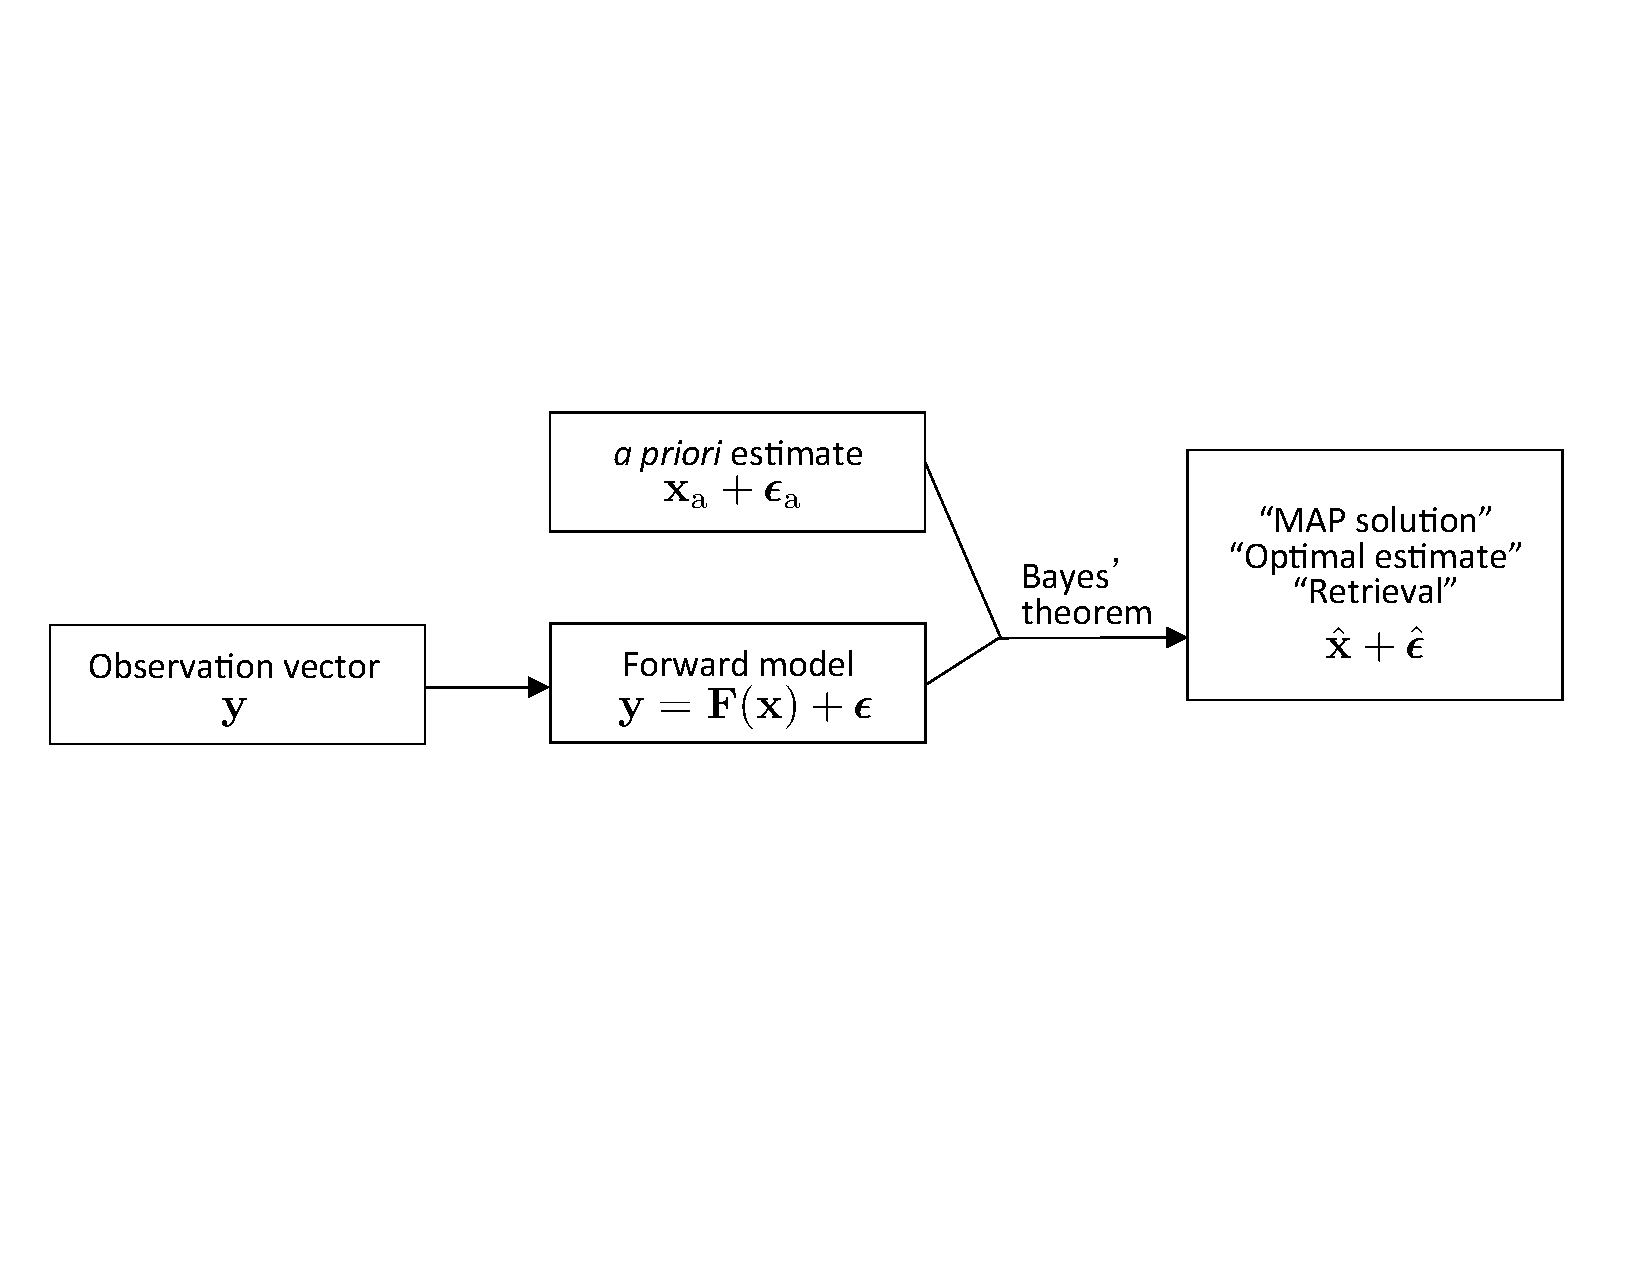
\includegraphics[width={0.9\textwidth}]{figures/MAP.pdf}
  \caption{The concept of an inverse problem that optimzing an estimates from observations. (Courtesy: Daniel Jacobs)}
  \label{fig:inversion}
\end{figure}

\subsection{Maximum a posteriori solution}
\subsection{Error characterization}
\subsection{Information theory}

\section{New Research Algorithm for AERONET Inversion}

General sturcture of the algorithm.

\subsection{Definition of state vector and Observation vector}
\subsection{Combine a priori and smoothness constraints}
\subsection{Statistical optimized inversion}
\subsection{Retrieval Error Characertization}
\subsection{Qaulity Control of Measurements}
